\documentclass[]{article}

\usepackage{graphicx}
\usepackage{Bookmark}

%opening
\title{Testing Document}
\author{Grant Louat}

\begin{document}

\maketitle

\begin{abstract}
This document details the testing of all functions, and their current state. Each function will be tested in isolation. This document should detail by what criteria the function has been deemed correct, the date and who did the testing. It should also have a listing of the working code so there is no confusion over different versions. This will quickly tell everyone which functions have been confirmed correct, and the rigour to which that assertion was made. It will also tell them when it was confirmed in case they have been working on a local copy of the code, and who deemed it correct in case they have questions. This document should also have a description of the function so that people know what the function should be doing when it is working.\newline
The document deals only with the isolation testing of each function. The functions will also need to be tested in an integration phase later.
\end{abstract}

\section{Common:}

\subsection{DIV\_X:}
\subsubsection{Status:}
Working as of 11:30 25/9/2014 - Grant

\subsubsection{Description:}
This set of Macros are designed to divide an integer by a power of two.

\subsubsection{Criteria:}
The value of 1024 was tested for each of the macros, and due to the simplicity and nature of the macros no other values need be tested.

\subsubsection{Working code:}
\#define DIV\_2(v) ((v) \>\> 1)       //Divide by 2

\section{Temperature Module:}

\subsection{ReadTempx2:}

\subsubsection{Status:}
Currently untested as of 8am 26/9/14 - Grant

\subsubsection{Description:}
Returns the temperature (x2) in degrees Celsius by performing an A/D conversion on the analogue output from the temperature sensor.

\subsection{ReadTemp:}
\subsubsection{Status:}
Working as of 8am 26/9/2014 - Grant

\subsubsection{Criteria:}
This function was tested in isolation of the ReadTempx2, and the assertion only applies to this function. A ReadTempx2 stub function was written to simply return the value of 40 to test the ReadTemp function.

\subsubsection{Description:}
The function simply calls the ReadTempx2 function and divides the result by 2.

\subsubsection{Working Code:}
unsigned char readTemp(void)
{
	unsigned char temp;
	
	temp = readTempx2();
	
	return DIV\_2(temp);
}

\subsection{RawTemp:}

\subsubsection{Status:}
Working as of 8:30am 26/9/2014 - Grant

\subsubsection{Criteria:}
The function was tested in isolation of the ReadTemp functions. A dummy function placed the value of 60 into the lastTempx2 variable, and the RawTemp function worked as described.

\subsubsection{Description:}
This function returns the uncalibrated result of the last temperature read. E.g. the raw sensor output. A temperature read is performed by either a ReadTemp or ReadTempx2 call. \newline:
This function cannot be completely tested in isolation as it requires an external static declaration of the lastTempx2 variable. It also requires the ReadTemp and ReadTempx2 functions to write to this variable when they perform a read.

\subsubsection{Working Code:}
unsigned char rawTemp(void)
{
	return DIV\_2(lastTempx2);
} 

\subsection{Calibrate Temp:}
\subsubsection{Status:}
Working as of 10:30am 26/9/2014 - Grant

\subsubsection{Description:}
Calibrates the last temperature read to the passed reference value by updating a static variable.

\subsubsection{Criteria:}
This function was tested in isolation of the readTemp functions. a dummy readTempx2 function which just returned 15deg (and set the static variable) was written, and the calibration function called to calibrate it to 20 deg, and then 10 deg. In both cases a second call of readTempx2 returned the desired value even though the 'raw data' was simply hard coded in.

\subsubsection{Working Code:}
void calibrateTemp(unsigned char reference)
{
	calibration\_offset = 2 * (reference - DIV\_2(lastTempx2));
}

\subsection{GetTemp:}

\subsubsection{Status:}
Working as of 10:30 26/9/2014 - Grant

\subsubsection{Description:}
Returns the result of the last temperature read.

\subsubsection{Criteria:}
This is just an accessor function, so it simply returns the value of a static variable.

\section{Range}

\subsection{SPD\_SND Macro}
\subsubsection{Status:}
Working as of 10:30 25/9/14 - Grant

\subsubsection{Description:}
This macro uses integer operations, so merely approximates the actual value to avoid lengthy floating point operations. 

\subsubsection{Criteria:}
Each temperature from 0 to 100 deg C was tested and compared to the actual formula result. There is some deviation due to the exclusive use of integer operations, but negligible See Fig. \ref{fig:SND_comp}.\newline 

\subsubsection{Working Code:}
\#define SPD\_SND(T) (DIV\_128(332 * (unsigned int)sqrt(16384 + T * (unsigned int)60)))

\begin{figure}
\centering
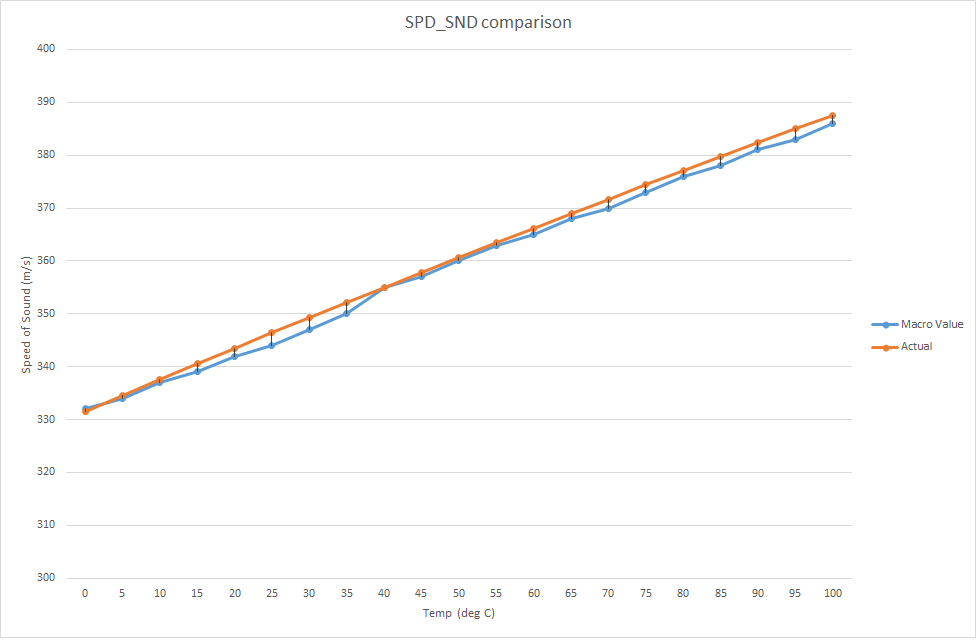
\includegraphics[width=0.7\linewidth]{../../../../../Pictures/SND_comp}
\caption{Comparison between SPD\_SND() Macro output and actual function value}
\label{fig:SND_comp}
\end{figure}


\end{document}
